Having outlined the methodology for using neural networks to solve differential equations, in this 
section, we begin a more systematic investigation of their performance across a range of ODE problems.
This section is divided into two main parts: initial value problems (IVPs) and boundary value problems
(BVPs). In each case, we examine the extent to which neural networks can learn accurate solutions 
and how their performance is affected by architectural choices.

In the IVP setting, we consider three representative classes of problems: exponential decay,
periodic solutions, and solutions containing a singularity. These problems allow us to assess 
both interpolation accuracy and a network's ability to extrapolate beyond the training domain.

For BVPs, our focus will remain on evaluating the quality of the approximation within the 
prescribed domain. Since boundary conditions are enforced at fixed endpoints, extrapolation 
beyond the interval is not typically meaningful. Instead, we investigate how the network adapts
to constraints at both boundaries, and how well it captures internal behaviour with different
choices of architecture and optimisation.

To systematically explore the influence of key design parameters, for each problem, we will vary: 
the number of neurons per hidden layer, the number of hidden layers and the choice of activation 
function. These experiments will serve to assess neural networks' ability to solve differential 
equation problems, along with understanding how this ability varies with architectural choices. 
We do not consider networks with different numbers of neurons in each layer, and we use the MSE
loss function for all models. We choose between the $\tanh$ and ReLU activation functions,
these being two of the most common activation functions chosen \cite{goodfellow2016deep}, 
and use the same activation functions in all networks, as is standard practice \cite{goodfellow2016deep}.

We deliberately restrict our investigation to variations in network architecture and activation 
functions, holding other hyperparameters fixed (such as the learning rate, optimiser type, and 
penalty parameters for enforcing boundary conditions). This choice simplifies the analysis and 
enables a clearer interpretation of the results by isolating the effects of architectural design. 
Our primary interest lies in the representational capability of neural networks — that is, how 
well different architectures can approximate solutions once trained — rather than in training 
efficiency. Provided that convergence is achieved, changes to hyperparameters like the learning 
rate or penalty weight primarily influence the speed or stability of training and not the final quality 
of the fit. To this end, we use the Adam optimiser, which is widely regarded as robust to 
hyperparameter settings such as the learning rate and penalty weight (\cite{goodfellow2016deep},
Section 8.5.4). To ensure fairness and comparability, all models were trained for the same 
number of epochs (typically 2500) with 100 training points in the domain, plus the 
boundary/initial value points. A learning rate of $\alpha = 0.001$ and penalty weight 
$\gamma = 100$ were used. All 
models were implemented in Python using the PyTorch library \cite{paszke2017automatic}.


\subsection{Initial Value Problems}\label{sec:IVPs}

\subsubsection{Exponential Decay}

We begin our analysis with a simple initial value problem whose solution exhibits exponential decay:
\[
\begin{aligned}
    y'(x) &= -y(x), \\
    y(0) &= 1.
\end{aligned}
\]
The exact solution is \( y(x) = e^{-x} \), a smooth and monotonic function defined on the entire real
line. This problem provides a natural baseline for assessing the ability of neural networks to 
approximate well-behaved solutions and to generalise beyond the training interval.

We train a series of feedforward neural networks on this problem using the architectural variation 
strategy described previously. Results for 
both \(\tanh\) and ReLU activation functions are shown in Figure~\ref{fig:expdecay_sidebyside}, 
including error heatmaps and examples of the best and worst performing networks under each 
activation function.

\begin{figure}[htbp]
    \centering
    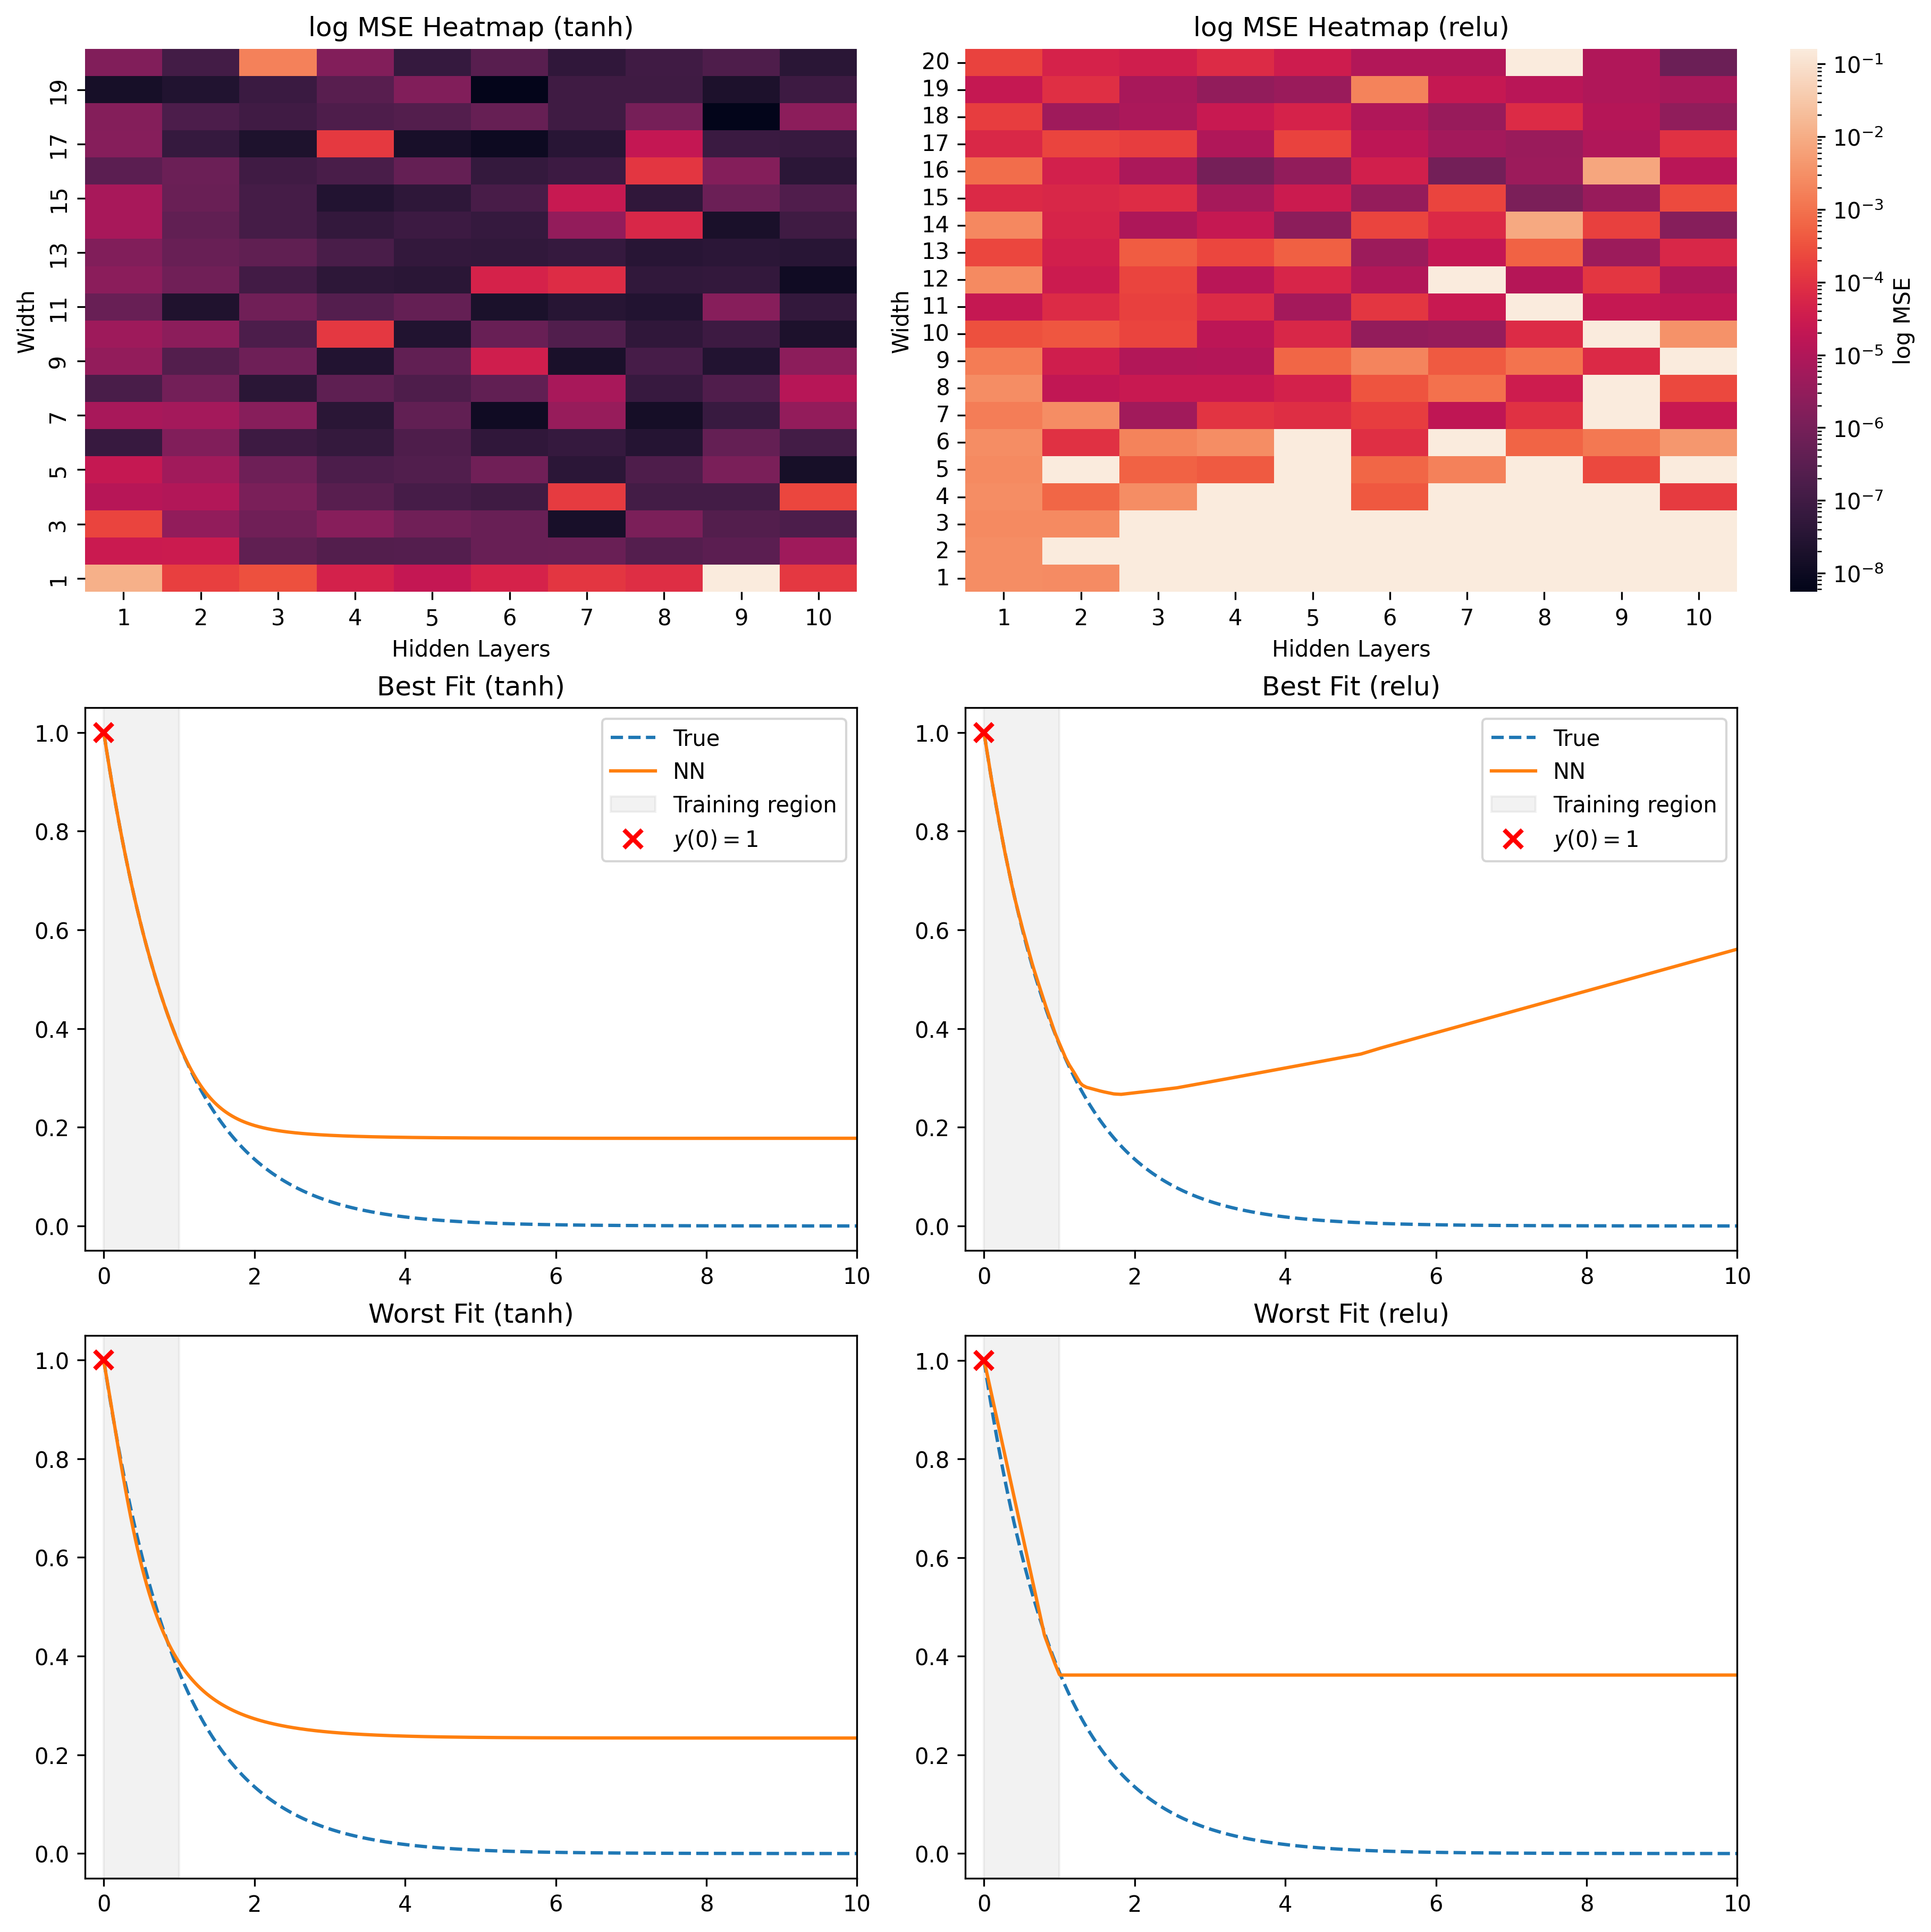
\includegraphics[width=\textwidth]{graphics/ivp_exponential_combined.png}
    \caption{Comparison of architectural performance for the exponential decay problem using two 
    activation functions. Each column shows the MSE heatmap with a log error scale,
    the best network fit, and the worst network fit.}
    \label{fig:expdecay_sidebyside}
\end{figure}


The heatmaps in Figure~\ref{fig:expdecay_sidebyside} reveal several consistent trends. For 
both activation functions, increasing the number of neurons per layer leads to improved 
accuracy for a fixed number of layers. In contrast, increasing depth alone did not guarantee better 
performance, particularly when layers are narrow. The best-performing configurations are found with 
moderately deep networks (4--8 layers) and wider layers (10--20 neurons), though the overall 
sensitivity to architecture is relatively mild, likely due to the simplicity of the target 
function. More striking differences emerge in extrapolation. The ReLU-based networks fail to 
capture the exponential decay beyond the training domain, typically reverting to a linear 
trajectory. By contrast, the networks trained with \(\tanh\) not only interpolate more accurately 
even in the worst case, but also exhibit qualitatively correct exponential behaviour when extrapolated 
to \(x = 10\). Finally, we observe in our heatmap that the error for most neural network architectures 
using the $\tanh$ activation function has lower MSE than those using the ReLu function, regardless 
of architecture, suggesting that the choice of activation function is a key determinant of quality of 
fit.



\subsubsection{Periodic Solution}

We now consider an initial value problem whose solution is periodic:
\[
\begin{aligned}
    y'(x) &= \cos x, \\
    y(0) &= 0.
\end{aligned}
\]
The exact solution is \( y(x) = \sin x \), which is smooth, bounded, and periodic with period \( 2\pi \).  
This problem allows us to evaluate the capacity of neural networks to approximate oscillatory behaviour
across a wide domain, and to generalise that behaviour beyond the domain.  

We perform the same analysis as in the previous section, first analysing how the error varies
for different architectures, and then examining the best solutions (we exclude the worst 
cases from now, as these were purely for comparison in the preceding section), shown in Figure 
\ref{fig:ivp_periodic_sidebyside}.

\begin{figure}[h]
    \centering
    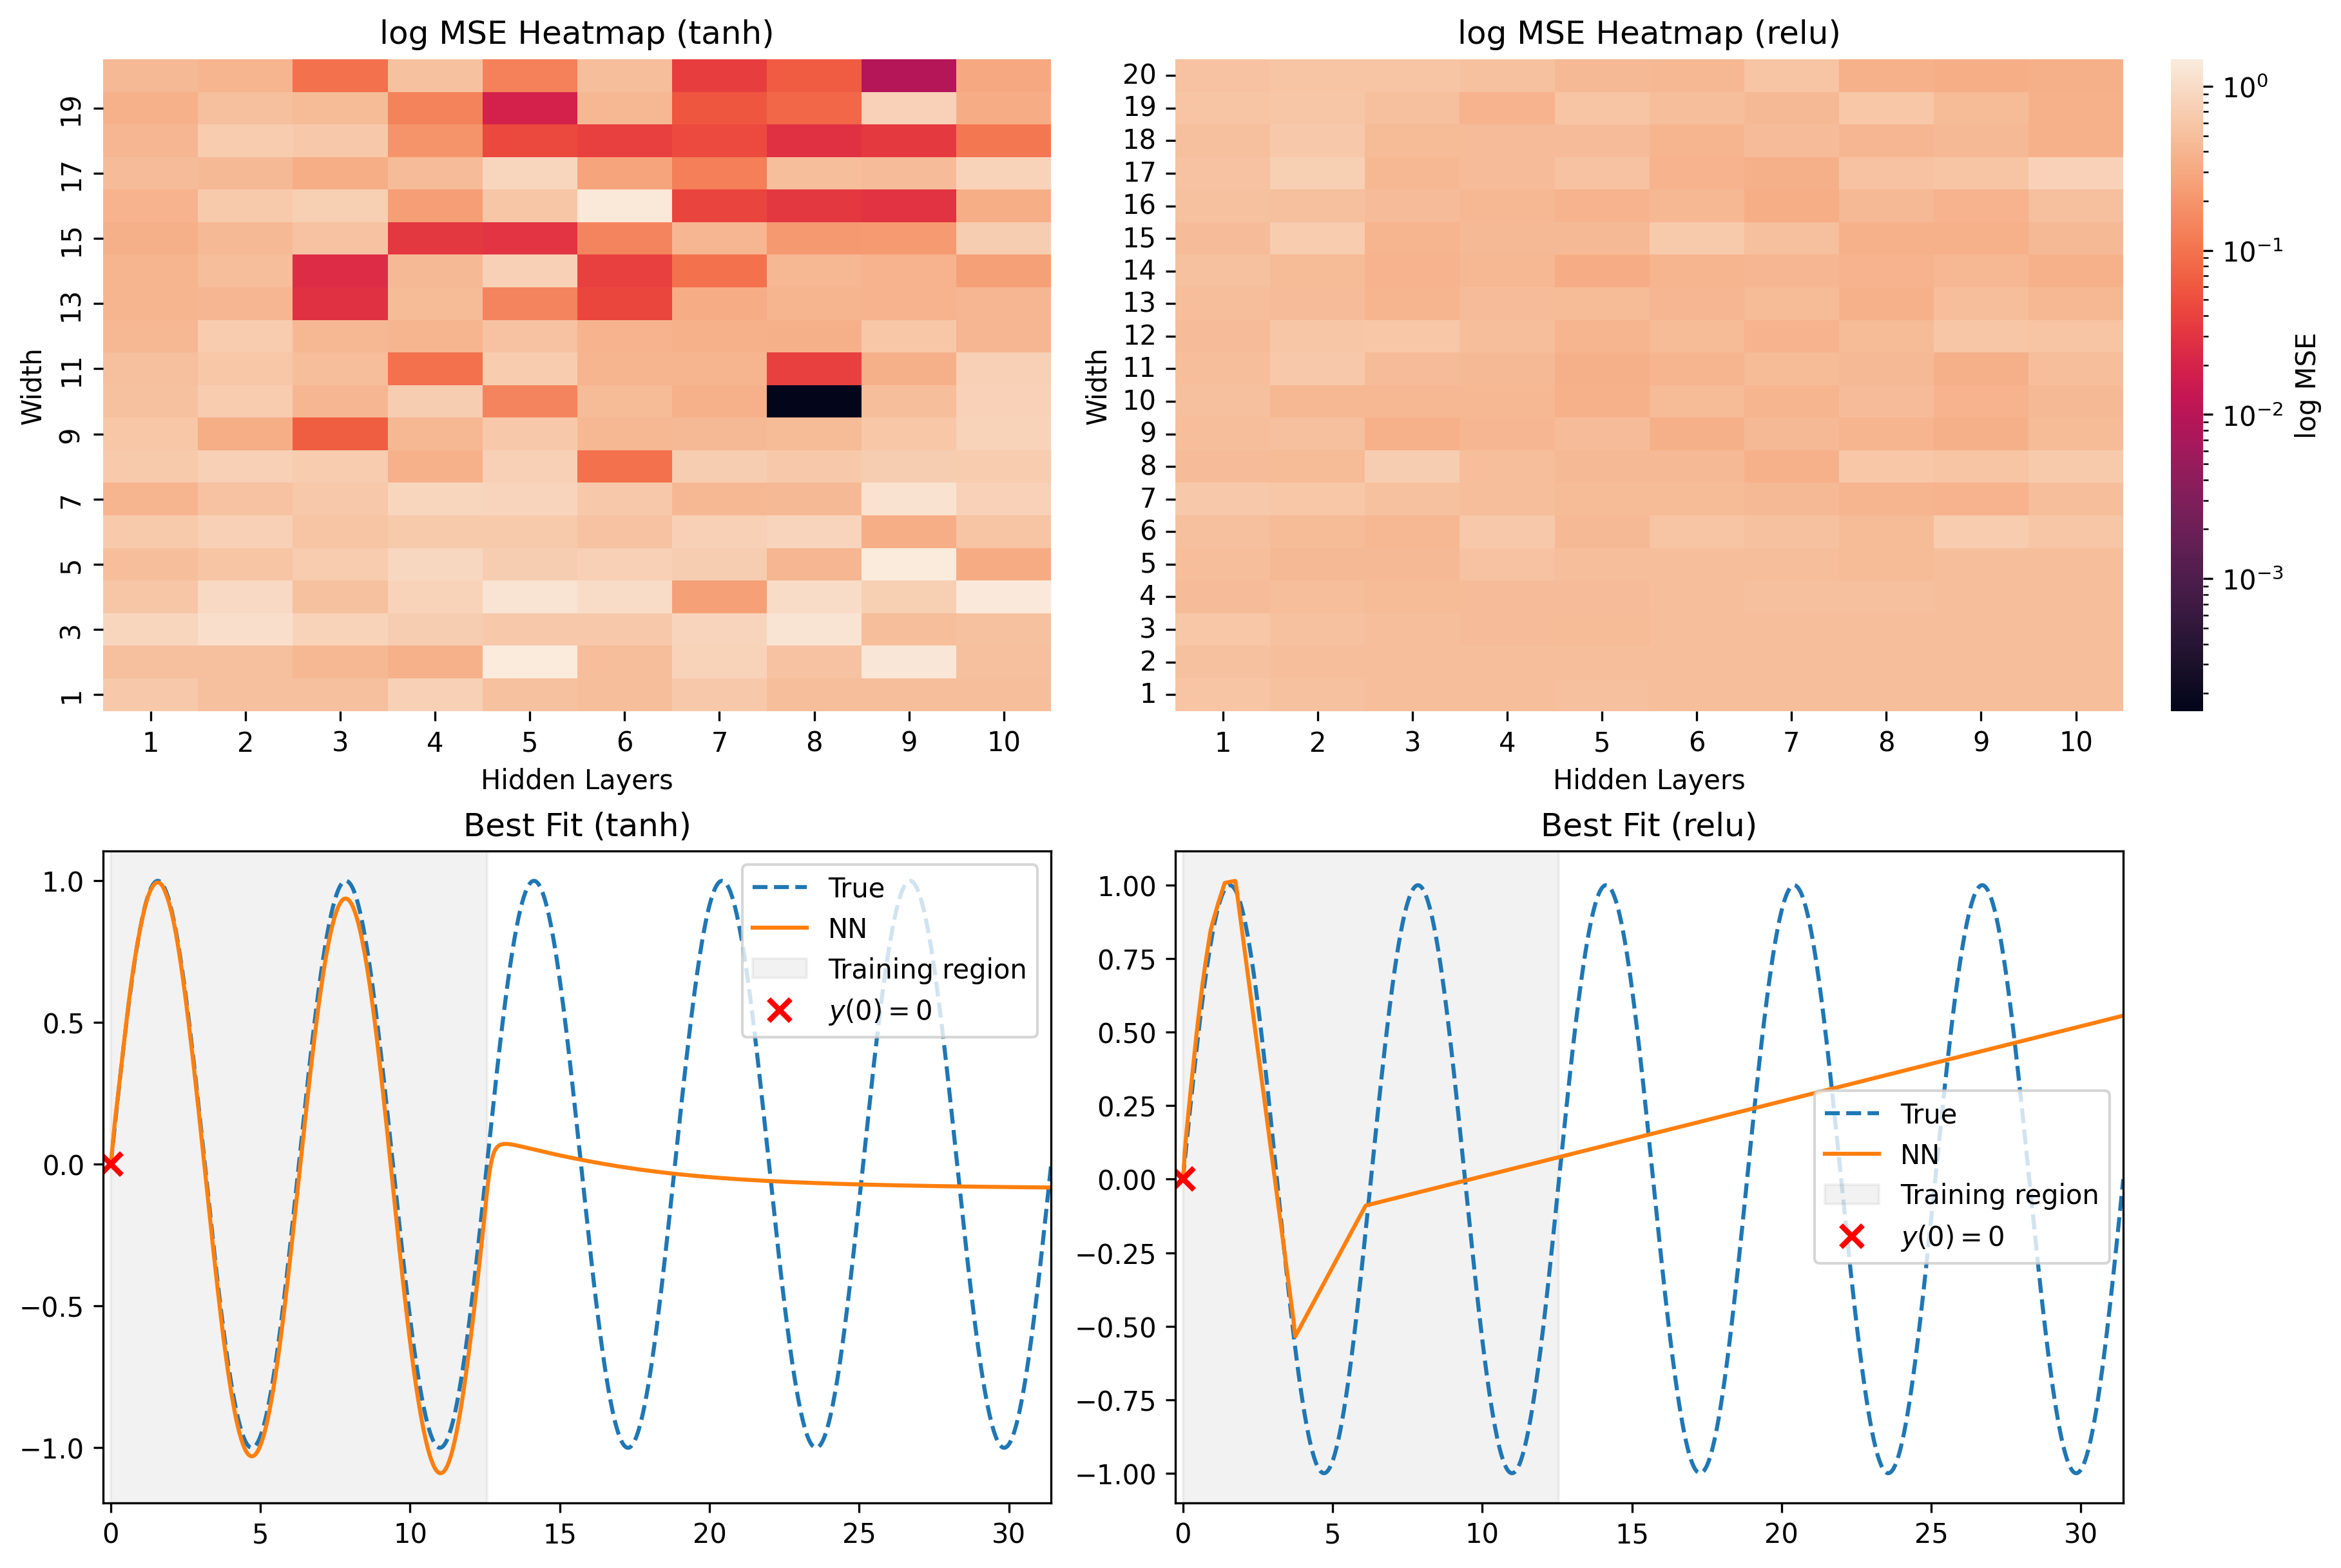
\includegraphics[width=\textwidth]{graphics/ivp_periodic_combined.png}
    \caption{Comparison of architectural performance for the oscillatory problem using two 
    activation functions. Each column shows the MSE heatmap with a log error scale,
    the best network fit for each activation function.}
    \label{fig:ivp_periodic_sidebyside}
\end{figure}

We observe that the choice of activation function has a significant impact on the network's 
ability to approximate this solution, the ReLU networks seeing negligible improvements 
in fit as the architecture was varied, and the \(\tanh\) activation function yielding 
noticeably better fits than ReLU. This is intuitive: \(\tanh\) is smooth and nonlinear, 
sharing important qualitative features with \(\sin(x)\), while ReLU is only piecewise linear 
and lacks curvature. As such, we would expect ReLU networks to require substantially greater 
depth and width to match the expressivity of a \(\tanh\)-based network. 
Both activations struggle to extrapolate periodicity beyond the training domain.
The predicted solutions flatten outside the interval, rather than 
propagating sinusoidal behaviour.


\subsubsection{Singular Solution}

We now turn to an initial value problem whose solution contains a singularity:
\[
\begin{aligned}
    y'(x) &= y(x)^2, \\
    y(0) &= 1, \\
    y(1.05) &= -20
\end{aligned}
\]
The exact solution is \( y(x) = \frac{1}{1 - x} \), which becomes singular at \( x = 1 \). This 
problem is useful for testing the ability of neural networks to approximate rapidly varying functions 
and to capture solution blow-up within a finite domain.

To mitigate instability near the singularity, we train two separate networks: one on the interval 
\([0, 0.95]\) using the initial condition \( y(0) = 1 \), and one on the interval \([1.05, 2.0] \) 
using the condition \( y(1.05) = -20 \). This approach allows us to evaluate how 
well neural networks can approximate the solution on either side of the singularity without 
numerical breakdown. Results are shown in Figure \ref{fig:ivp_singular_sidebyside}.

\begin{figure}[h]
    \centering
    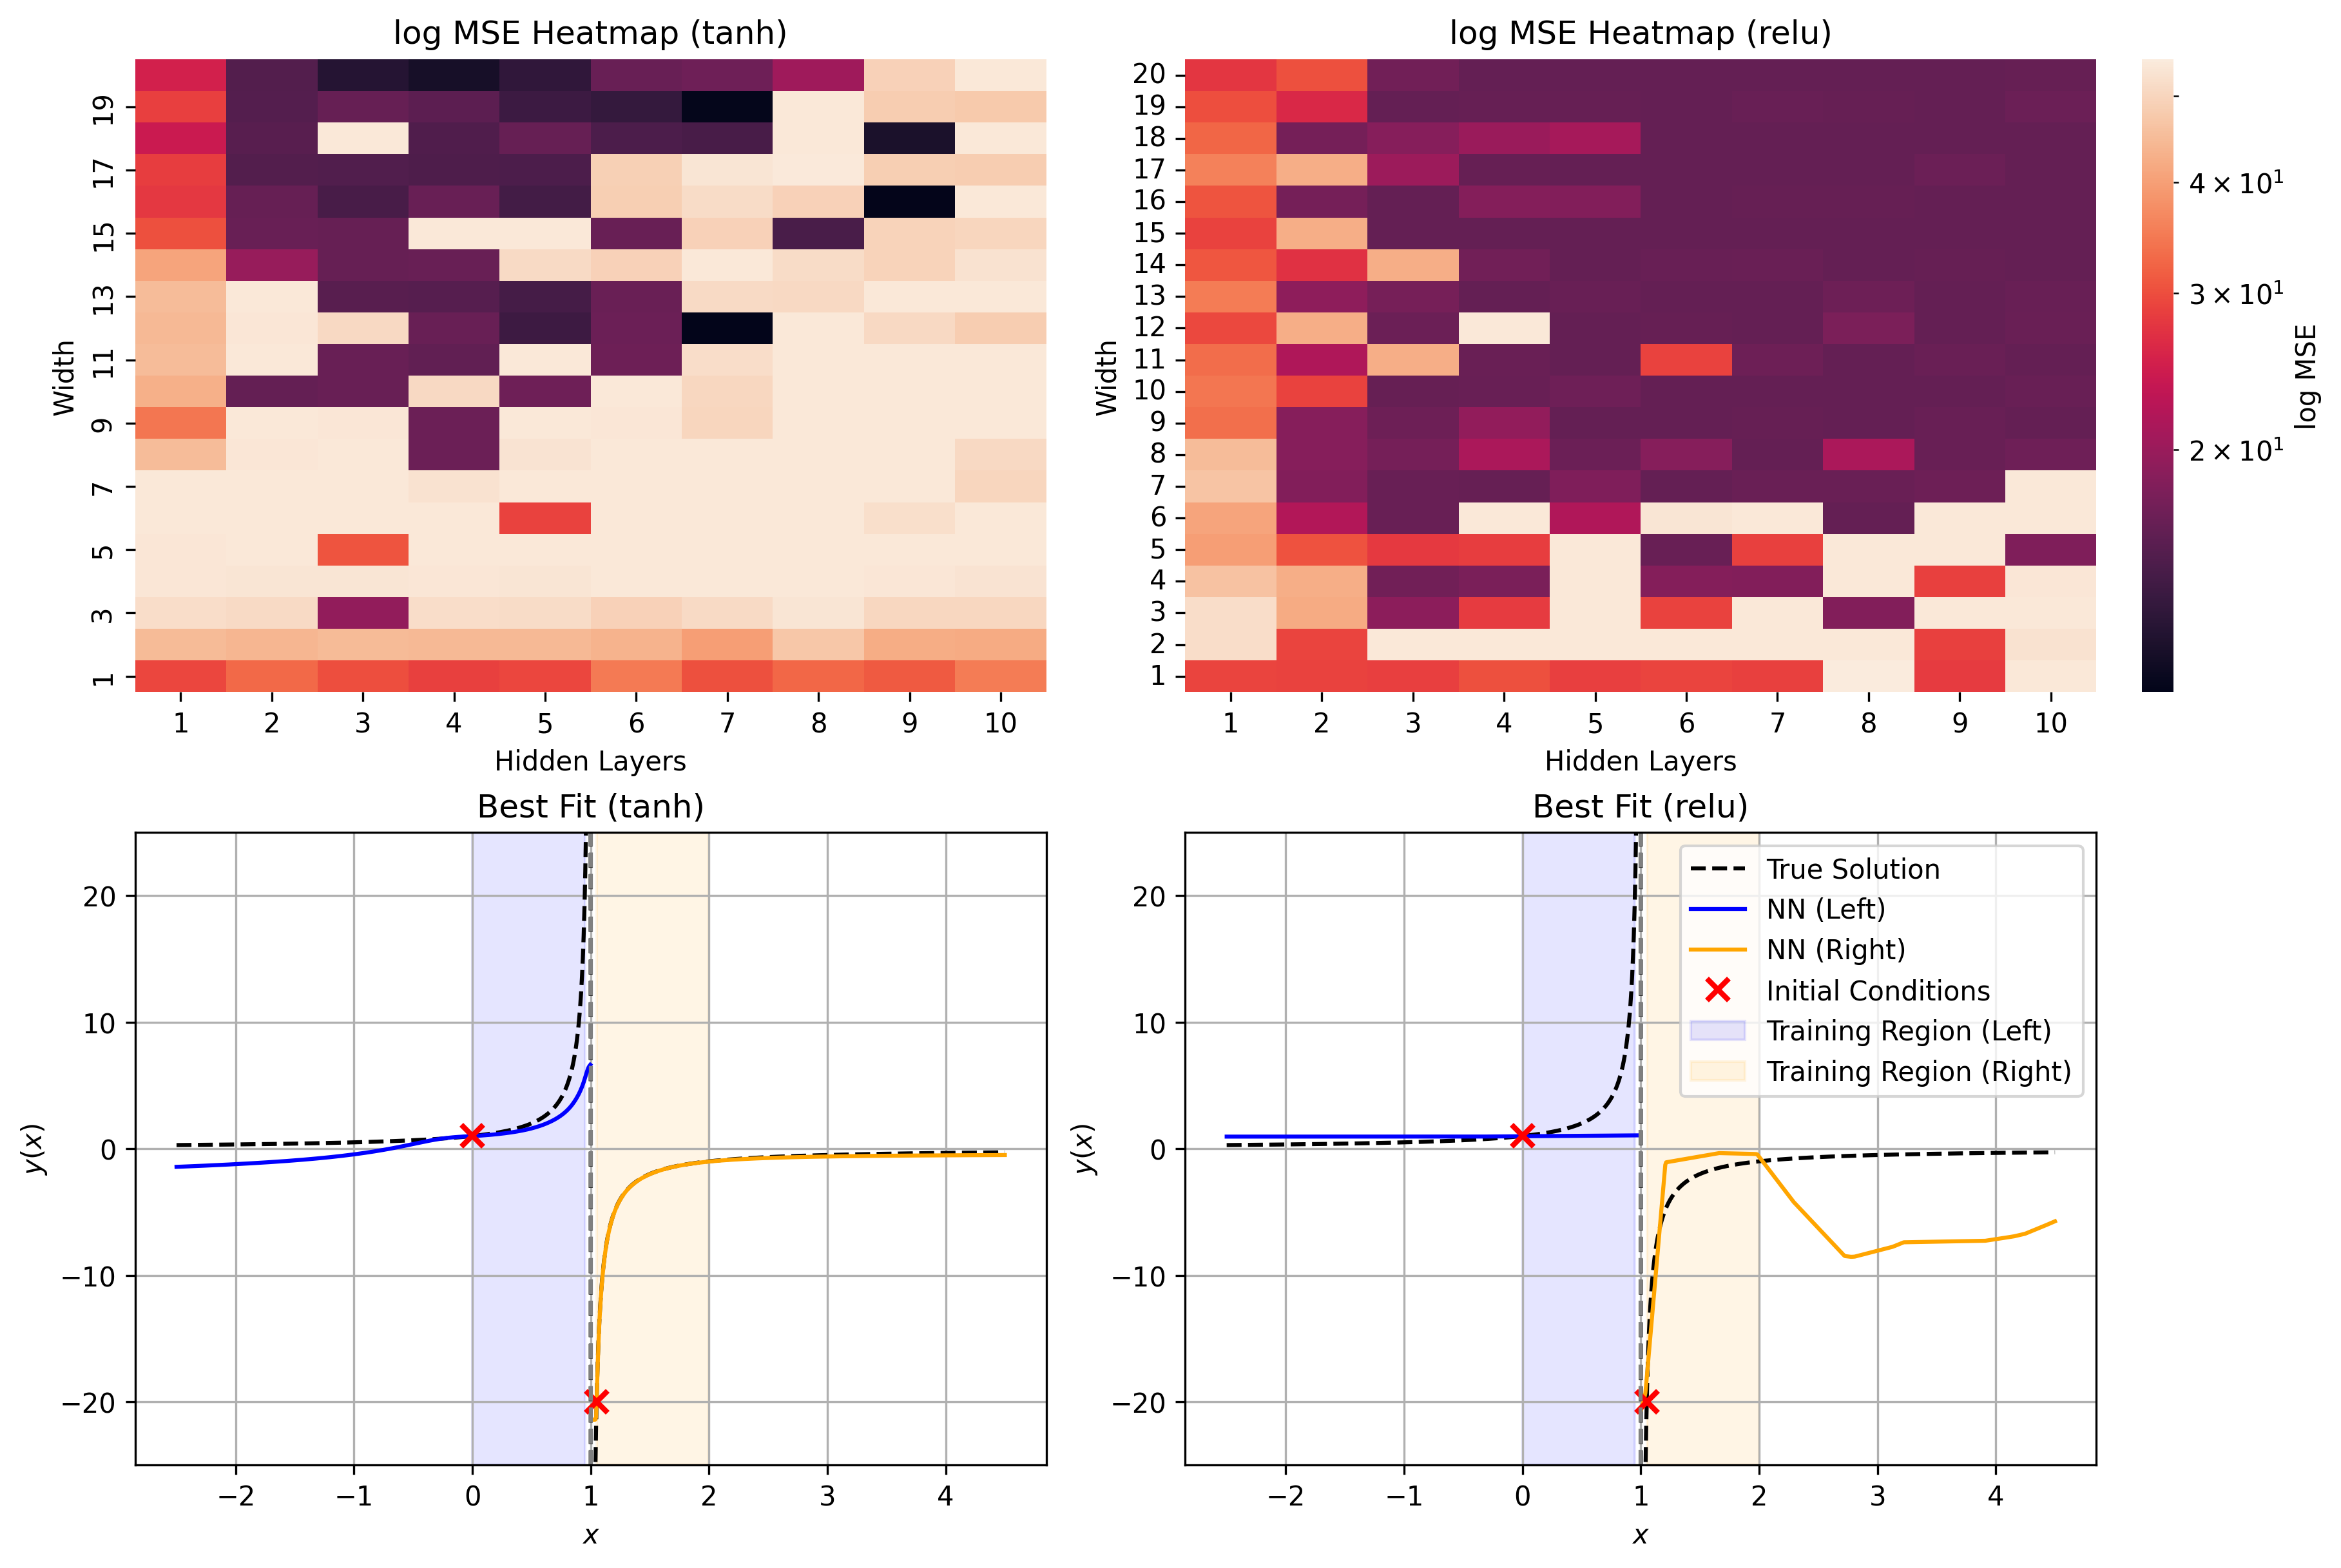
\includegraphics[width=\textwidth]{graphics/ivp_singularity_combined.png}
    \caption{Comparison of architectural performance for the singular solution problem using two 
    activation functions. Each column shows the MSE heatmap with a log error scale,
    the best network fit, and the worst network fit.}
    \label{fig:ivp_singular_sidebyside}
\end{figure}

Figure~\ref{fig:ivp_singular_sidebyside} shows that while the ReLU activation function yields 
lower MSE across a broader range of architectures, the \(\tanh\) activation achieves significantly
better fits for select configurations. Notably, networks using \(\tanh\) require at least 7 hidden 
layers to perform well, with accuracy dropping sharply for deeper architectures beyond 8 layers. 
An interesting pattern emerges with respect to width: networks with only one neuron per layer often 
outperform those with 2-3 neurons, suggesting that minimal width can sometimes aid in learning steep 
gradients near singularities. In terms of qualitative behaviour, the best \(\tanh\) network closely 
tracks the exact solution on the right side of the singularity and extrapolates smoothly beyond the 
training region, converging to a nearly linear continuation, while also beginning to capture the shape
on the left side. In contrast, the ReLU network produces jagged, piecewise responses outside the 
training domain, failing to capture the smooth decay, and completely failing 
to capture the structure on the left of the singularity.



\subsection{Boundary Value Problems}\label{sec:BVPs}


We now consider boundary value problems (BVPs), where the solution is defined by a 
differential equation along with prescribed values at the boundaries of a fixed domain. Unlike 
initial value problems, BVPs specify constraints at multiple points—typically at the endpoints of 
an interval—and the solution must satisfy the differential equation throughout the domain while 
adhering to these boundary conditions.

In this section, we investigate how well neural networks can approximate solutions to BVPs using 
the same methodology outlined for IVPs. However, since BVPs are defined strictly on a bounded 
interval, we do not consider extrapolation performance here. Instead, we focus on how accurately 
the networks capture the solution within the specified domain.

We consider two BVPs:
\begin{itemize}
    \item A smooth Poisson-type problem, with known analytic solution $y(x)=sin(\pi x)$, 
    serving as a baseline. 
    \item A piecewise forcing problem with a discontinuous right-hand side, used to examine network
     behaviour under more challenging conditions. 
\end{itemize}




\subsubsection{Poisson Problem}

We begin with a classical boundary value problem from mathematical physics:
\[
\begin{aligned}
    -y''(x) &= \pi^2 \sin(\pi x), \quad x \in (0, 1), \\
    y(0) &= 0, \\
    y(1) &= 0.
\end{aligned}
\]
This has the exact solution \( y(x) = \sin(\pi x) \), which is smooth, bounded, and vanishes at both 
endpoints. The problem provides a simple setting to evaluate how well neural networks approximate 
solutions to second-order differential equations with smooth forcing and well-defined boundary 
conditions, and how those approximations vary with architecture.

As in the IVP analysis, we assess the effect of architectural variation on solution accuracy.
For each combination of depth, width, and activation function, we compute the MSE across the domain,
and visualise the results using heatmaps and the best fits, shown in 
Figure~\ref{fig:bvp_poisson_sidebyside}.

\begin{figure}[h]
    \centering
    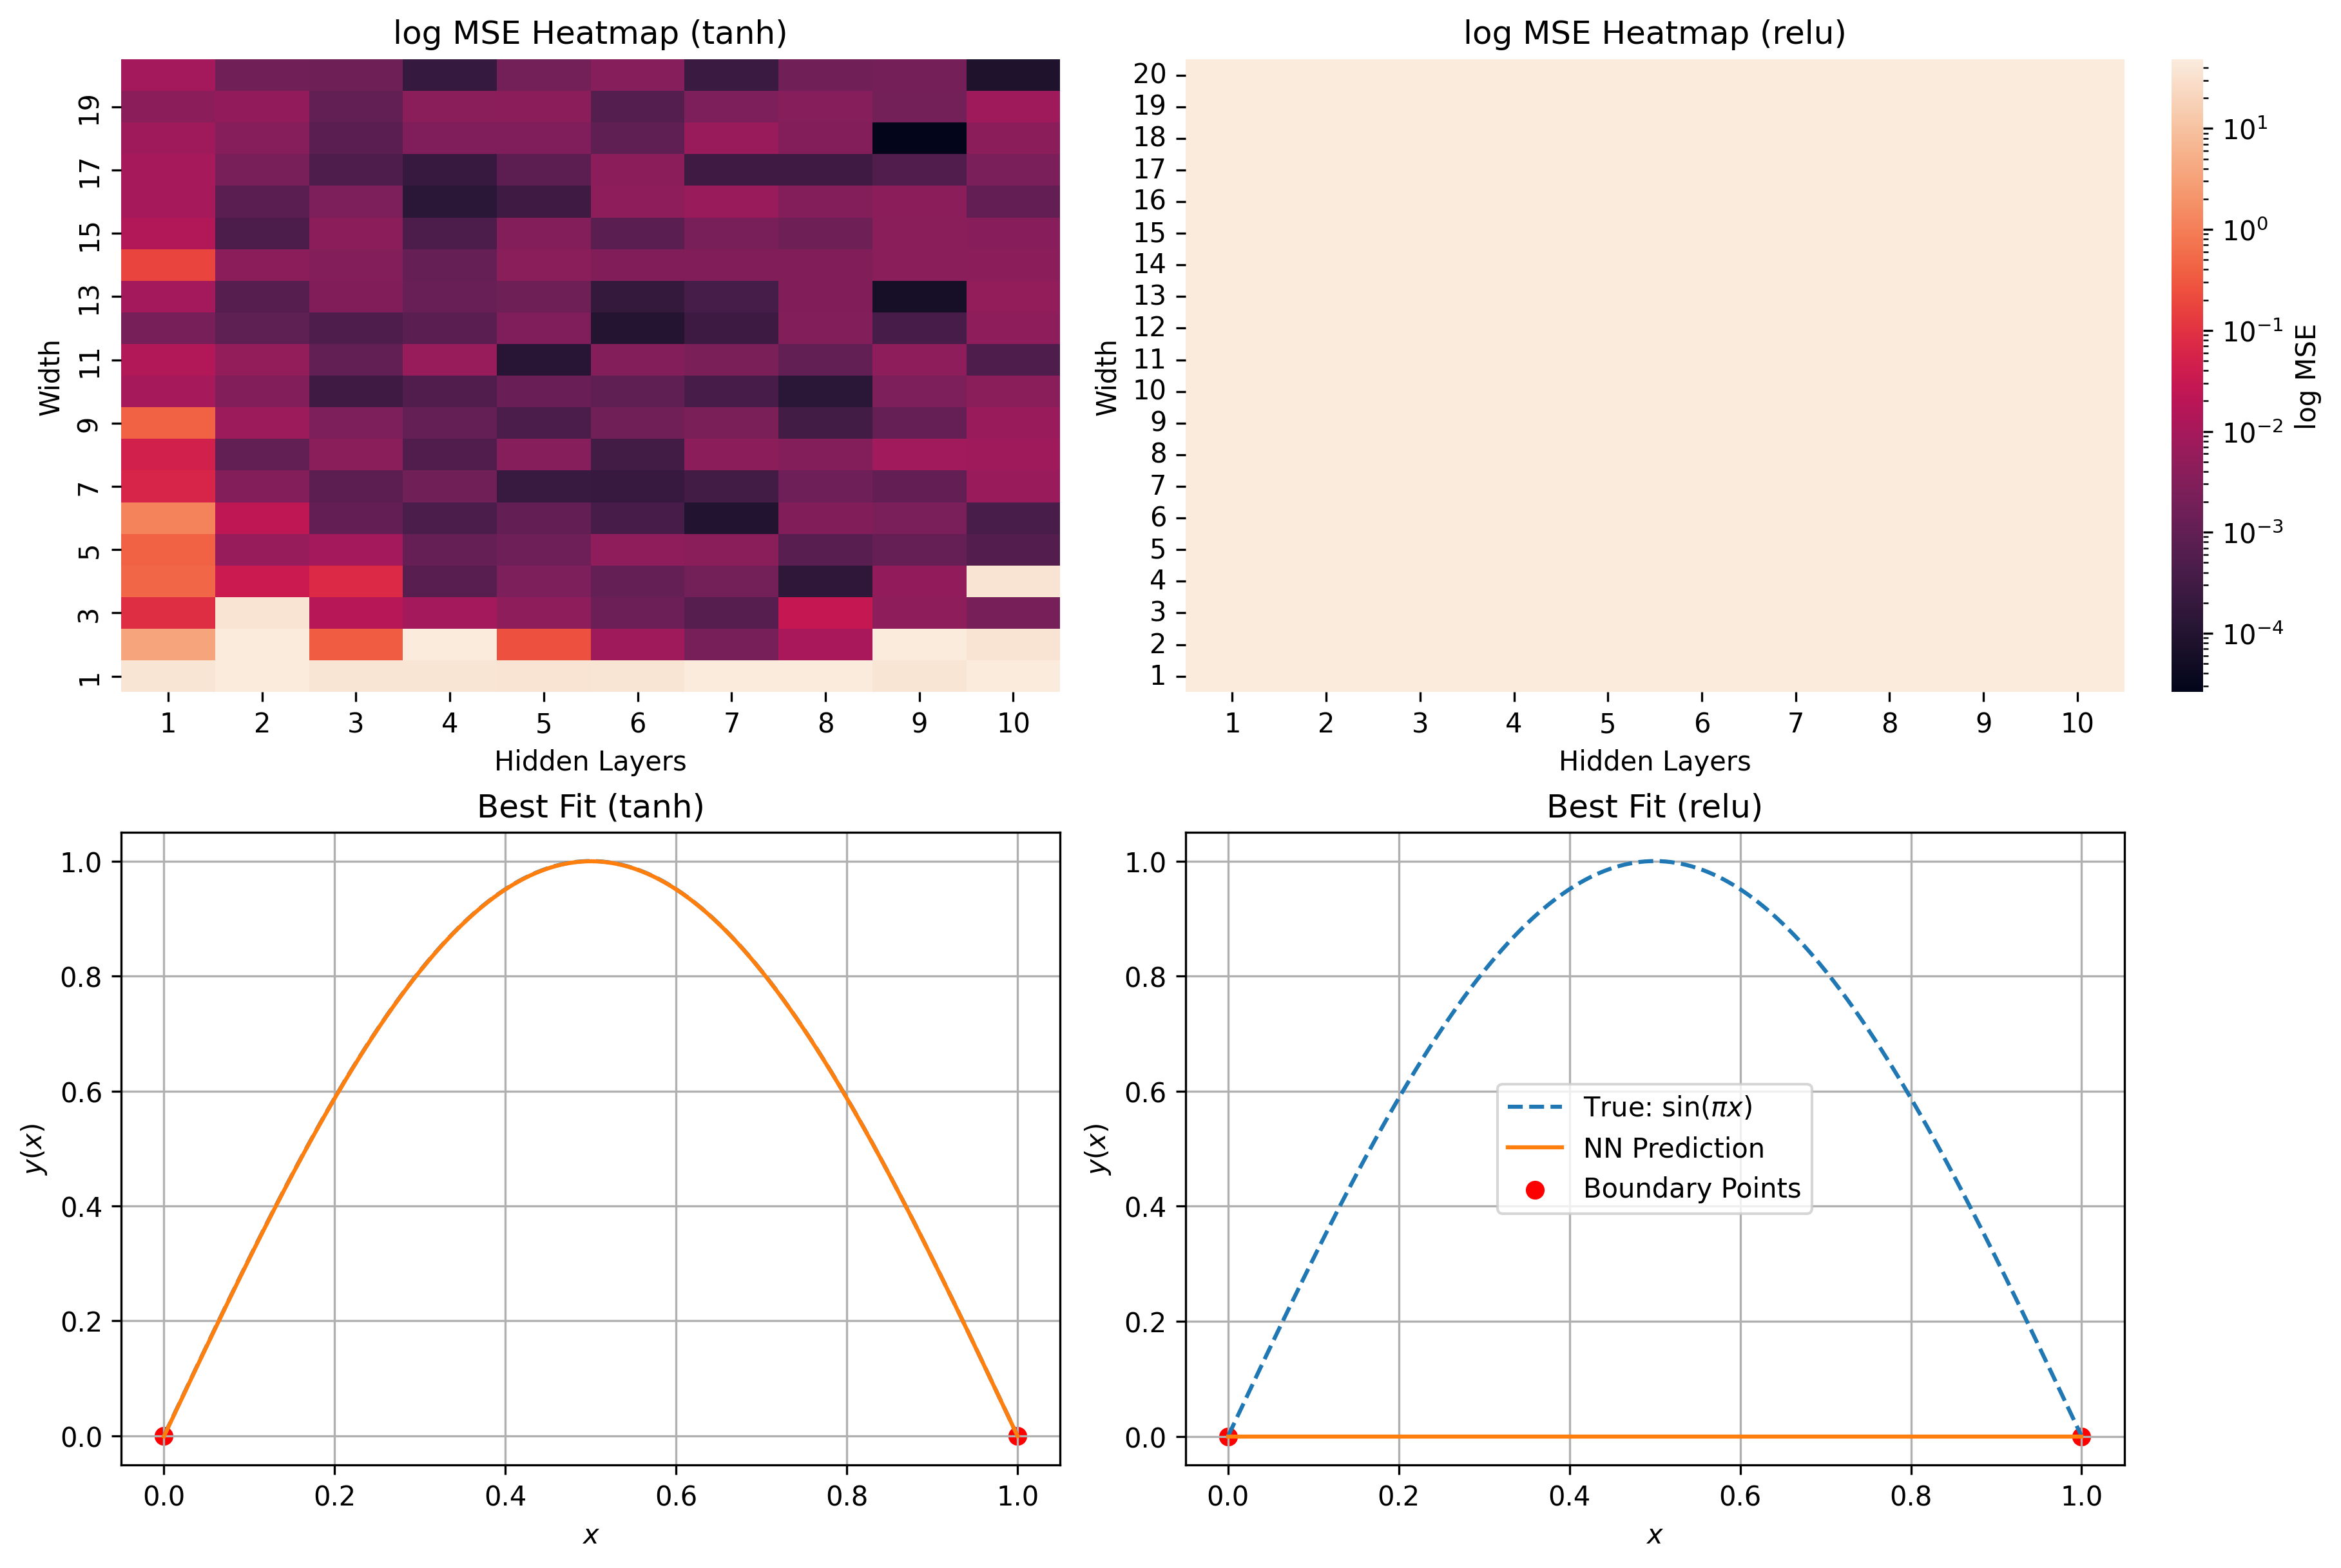
\includegraphics[width=\textwidth]{graphics/bvp_poisson_combined.png}
    \caption{Comparison of architectural performance for the Poisson BVP using two 
    activation functions. Each column shows the MSE heatmap with a log error scale,
    the best network fit, and the worst network fit.}
    \label{fig:bvp_poisson_sidebyside}
\end{figure}

The ReLU activation function exhibits a clear inability to capture the curvature of the solution 
in this problem. Across all tested architectures, it appears to reduce error primarily by satisfying
the boundary conditions, rather than accurately fitting the interior solution. In contrast, 
the $\tanh$ activation function consistently achieves an excellent approximation, with 
performance improving steadily as both depth and width are increased. This result is 
consistent with earlier observations, where $\tanh$ proved particularly well-suited to 
approximating sinusoidal solutions over the training domain.

\subsubsection{Piecewise Forcing}

We now consider a boundary value problem with a discontinuous right-hand side:
\[
\begin{aligned}
    y''(x) &= 
    \begin{cases}
        -1, & 0 \leq x < 0.5, \\
        +1, & 0.5 \leq x \leq 1,
    \end{cases} \\
    y(0) &= 0, \\
    y(1) &= 0.
\end{aligned}
\]
The exact solution is piecewise quadratic, continuous, and satisfies the boundary conditions. 
However, the discontinuity in the forcing term induces a derivative jump at \( x = 0.5 \), 
making this a challenging test case for smooth neural network approximators.

This example allows us to assess how well neural networks can adapt to discontinuous dynamics
in the governing equation. As before, we systematically vary network architecture and activation 
function, compute the corresponding approximation error, and visualise representative results.
The best-fitting solutions are summarised in Figure~\ref{fig:bvp_piecewise_sidebyside}.

\begin{figure}[h]
    \centering
    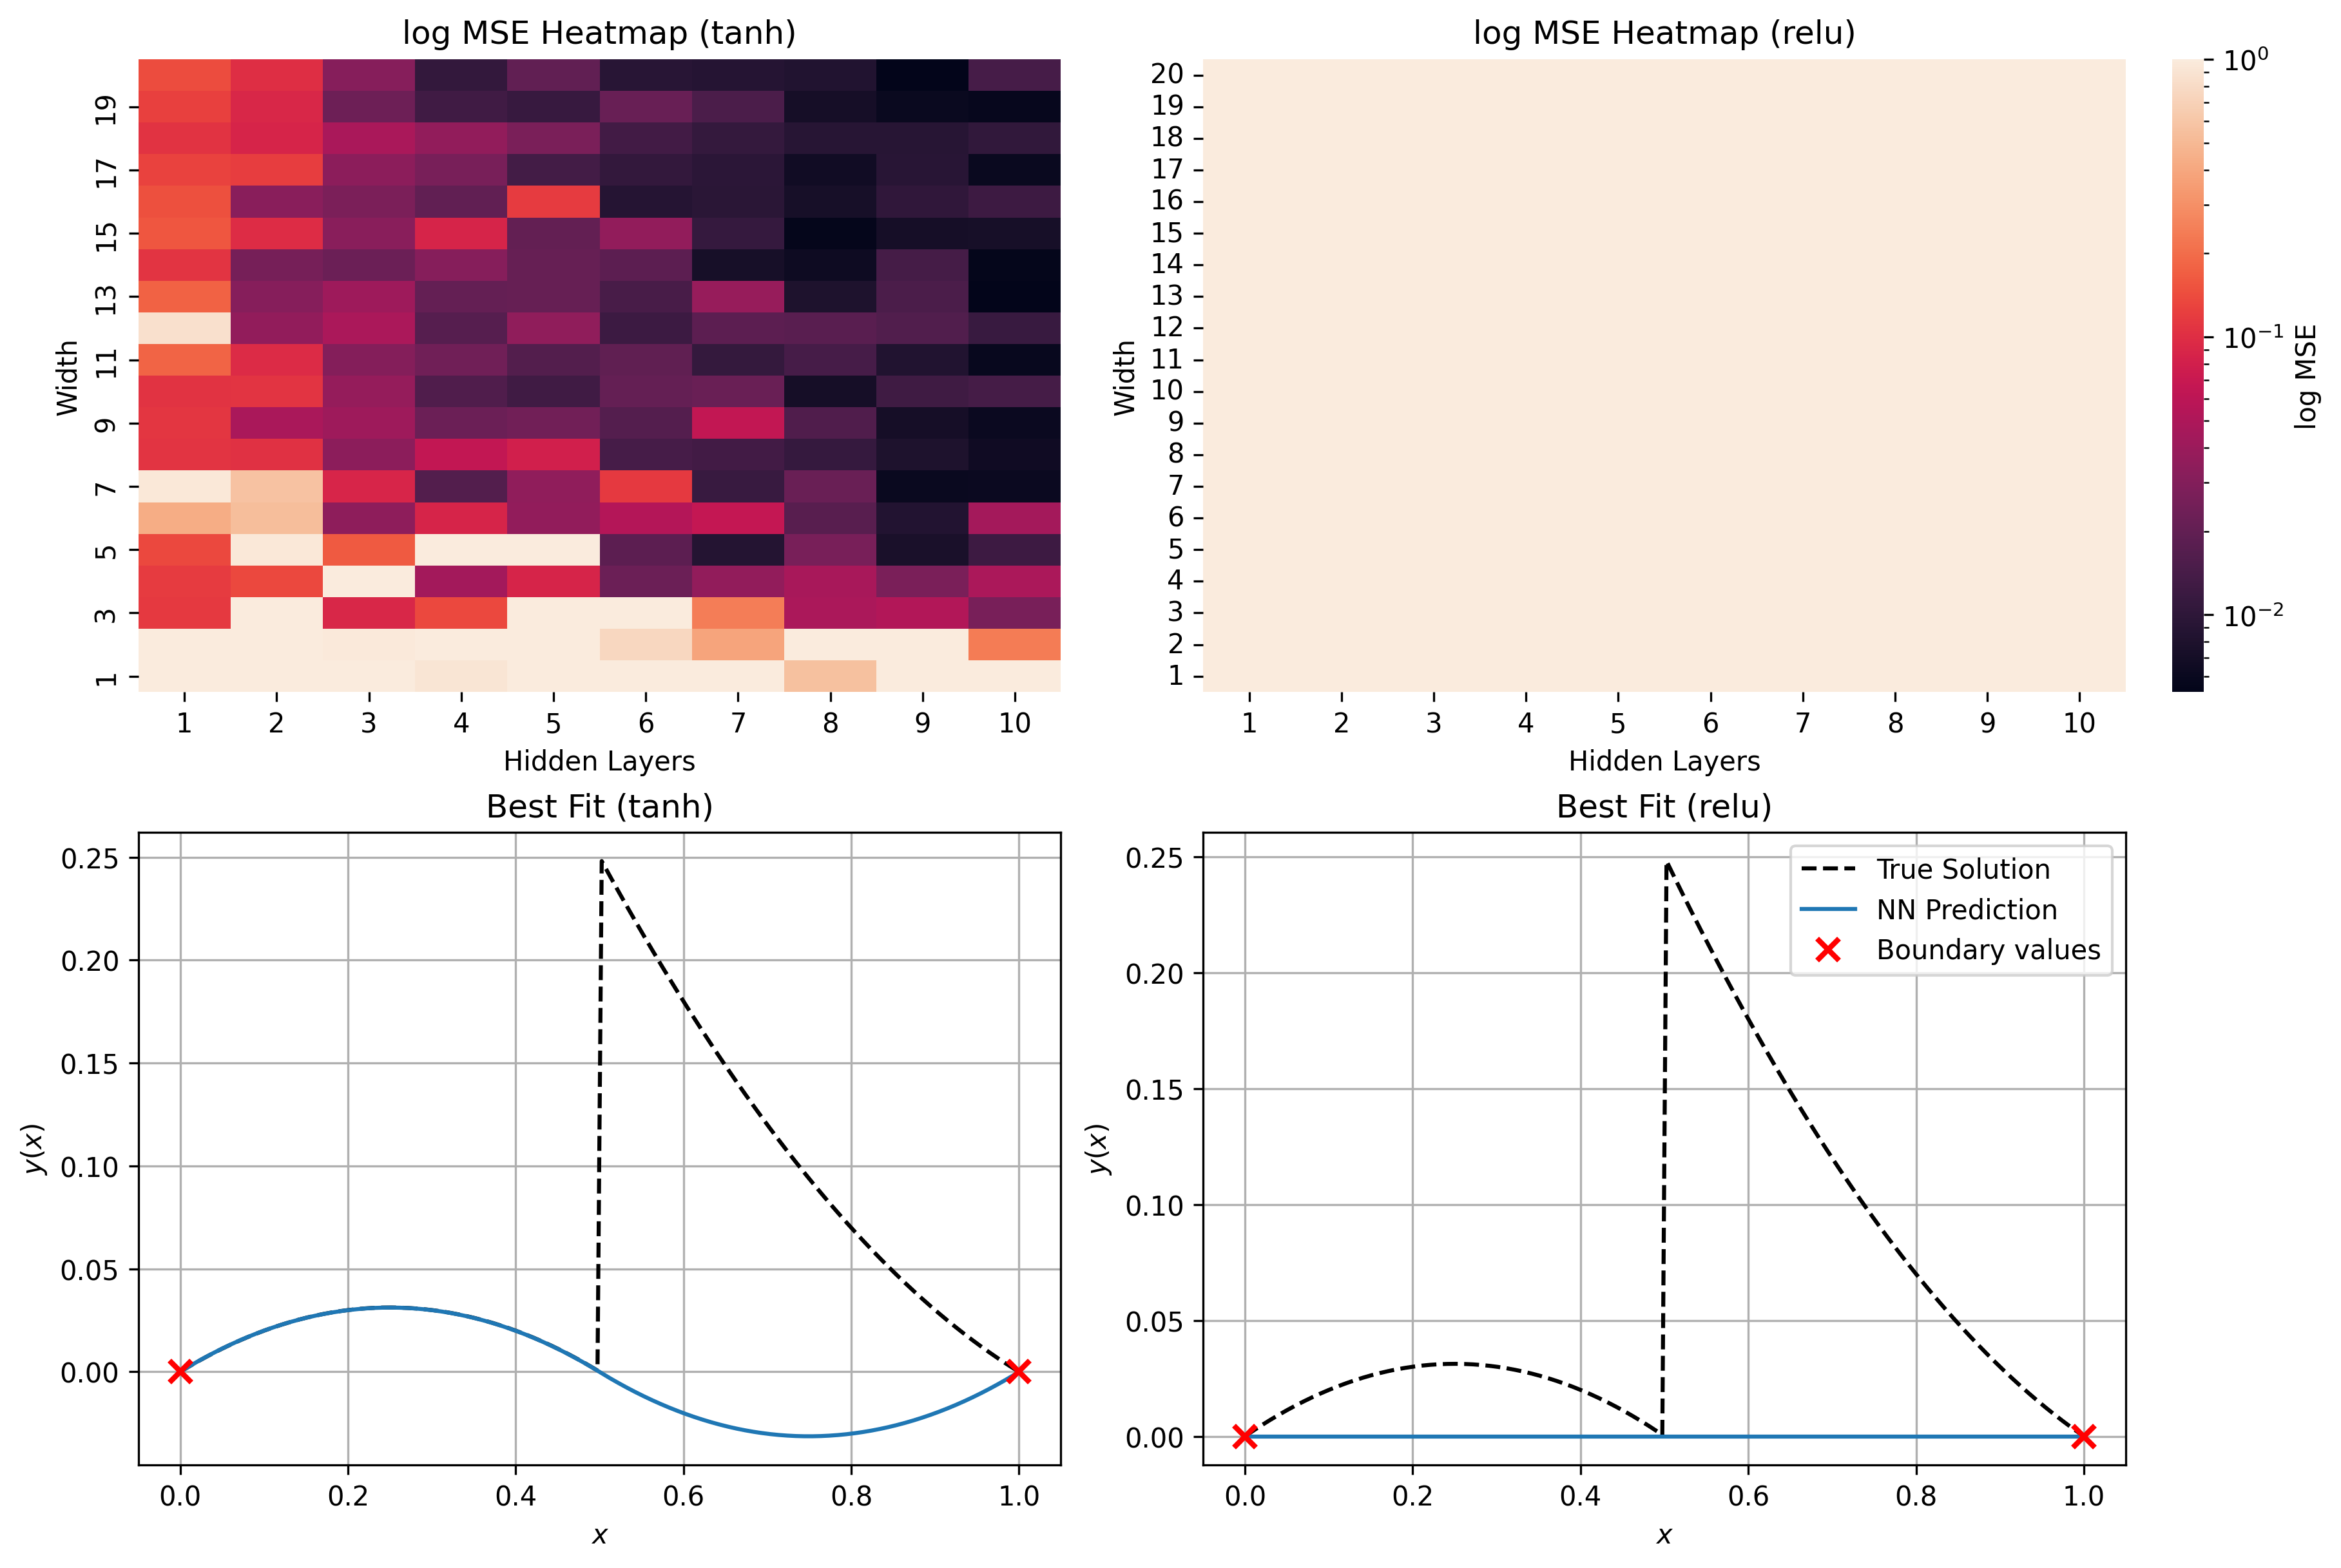
\includegraphics[width=\textwidth]{graphics/bvp_piecewise_combined.png}
    \caption{Comparison of architectural performance for the piecewise-forced BVP using two 
    activation functions. Each column shows the MSE heatmap (log scale) and best-fit solution.}
    \label{fig:bvp_piecewise_sidebyside}
\end{figure}

ReLU once again fails to capture the underlying structure of the solution, instead converging to a 
trivial fit that satisfies only the boundary conditions. In contrast, networks using the 
\(\tanh\) activation function show clear improvement with increased width and depth. 
Interestingly, rather than adapting to the discontinuity in the forcing term, the 
\(\tanh\) networks tend to converge toward smooth, sinusoidal-like approximations.
